%%
%% This is file `sample-manuscript.tex',
%% generated with the docstrip utility.
%%
%% The original source files were:
%%
%% samples.dtx  (with options: `all,proceedings,bibtex,manuscript')
%%
%% IMPORTANT NOTICE:
%%
%% For the copyright see the source file.
%%
%% Any modified versions of this file must be renamed
%% with new filenames distinct from sample-manuscript.tex.
%%
%% For distribution of the original source see the terms
%% for copying and modification in the file samples.dtx.
%%
%% This generated file may be distributed as long as the
%% original source files, as listed above, are part of the
%% same distribution. (The sources need not necessarily be
%% in the same archive or directory.)
%%
%%
%% Commands for TeXCount
%TC:macro \cite [option:text,text]
%TC:macro \citep [option:text,text]
%TC:macro \citet [option:text,text]
%TC:envir table 0 1
%TC:envir table* 0 1
%TC:envir tabular [ignore] word
%TC:envir displaymath 0 word
%TC:envir math 0 word
%TC:envir comment 0 0
%%
%% The first command in your LaTeX source must be the \documentclass
%% command.
%%
%% For submission and review of your manuscript please change the
%% command to \documentclass[manuscript, screen, review]{acmart}.
%%
%% When submitting camera ready or to TAPS, please change the command
%% to \documentclass[sigconf]{acmart} or whichever template is required
%% for your publication.
%%
%%
\documentclass[manuscript,screen,review]{acmart}
\usepackage{tikz}
\usetikzlibrary{positioning,arrows.meta}
%%
%% \BibTeX command to typeset BibTeX logo in the docs
\AtBeginDocument{%
  \providecommand\BibTeX{{%
    Bib\TeX}}}

%% Rights management information.  This information is sent to you
%% when you complete the rights form.  These commands have SAMPLE
%% values in them; it is your responsibility as an author to replace
%% the commands and values with those provided to you when you
%% complete the rights form.
% \setcopyright{acmlicensed}
% \copyrightyear{2025}
% \acmYear{2025}
% \acmDOI{XXXXXXX.XXXXXXX}
%% These commands are for a PROCEEDINGS abstract or paper.
% \acmConference[Conference acronym 'XX]{Make sure to enter the correct
%   conference title from your rights confirmation email}{June 03--05,
%   2018}{Woodstock, NY}
%%
%%  Uncomment \acmBooktitle if the title of the proceedings is different
%%  from ``Proceedings of ...''!
%%
%%\acmBooktitle{Woodstock '18: ACM Symposium on Neural Gaze Detection,
%%  June 03--05, 2018, Woodstock, NY}
% \acmISBN{978-1-4503-XXXX-X/2018/06}

%%
%% Submission ID.
%% Use this when submitting an article to a sponsored event. You'll
%% receive a unique submission ID from the organizers
%% of the event, and this ID should be used as the parameter to this command.
%%\acmSubmissionID{123-A56-BU3}

%%
%% For managing citations, it is recommended to use bibliography
%% files in BibTeX format.
%%
%% You can then either use BibTeX with the ACM-Reference-Format style,
%% or BibLaTeX with the acmnumeric or acmauthoryear sytles, that include
%% support for advanced citation of software artefact from the
%% biblatex-software package, also separately available on CTAN.
%%
%% Look at the sample-*-biblatex.tex files for templates showcasing
%% the biblatex styles.
%%

%%
%% The majority of ACM publications use numbered citations and
%% references.  The command \citestyle{authoryear} switches to the
%% "author year" style.
%%
%% If you are preparing content for an event
%% sponsored by ACM SIGGRAPH, you must use the "author year" style of
%% citations and references.
%% Uncommenting
%% the next command will enable that style.
%%\citestyle{acmauthoryear}


%%
%% end of the preamble, start of the body of the document source.
\begin{document}

%%
%% The "title" command has an optional parameter,
%% allowing the author to define a "short title" to be used in page headers.
\title{Predicting Biological Age of ICU Patients from MIMIC-IV Using TabM}

%%
%% The "author" command and its associated commands are used to define
%% the authors and their affiliations.
%% Of note is the shared affiliation of the first two authors, and the
%% "authornote" and "authornotemark" commands
%% used to denote shared contribution to the research.
\author{Elliot Farmer Garcia}
\email{efgarcia@utexas.edu}
% \orcid{1234-5678-9012}
\affiliation{%
  \institution{University of Texas at Austin}
  \city{Austin}
  \state{Texas}
  \country{USA}
}

%%
%% By default, the full list of authors will be used in the page
%% headers. Often, this list is too long, and will overlap
%% other information printed in the page headers. This command allows
%% the author to define a more concise list
%% of authors' names for this purpose.
\renewcommand{\shortauthors}{Farmer Garcia}

%%
%% The abstract is a short summary of the work to be presented in the
%% article.
\begin{abstract}
Estimating a patient’s biological age from routinely collected ICU data offers a window into physiologic reserve and potential trajectories in critical care. We curate a cohort of 72\,338 ICU admissions from MIMIC-IV, extracting 33 features—including demographics (gender, insurance, language, marital status, race), length of stay, and admission-averaged vital signs and laboratory measurements. Missing categorical values are imputed using the most frequent category and encoded ordinally, while continuous variables are imputed via KNN ($k=5$) and standardized. We compare a simple multilayer perceptron (MLP) baseline against TabM, a lightweight BatchEnsemble MLP, both with and without categorical inputs. On a held-out validation set, the MLP baseline achieves an RMSE of $11.28\,$years, TabM without categorical inputs yields an RMSE of $11.04\,$years, and TabM with categorical inputs reduces RMSE to $9.24\,$years—an $\approx18\%$ reduction relative to the baseline. These results demonstrate that TabM, when paired with principled imputation and categorical encoding, yields a promising biological-age predictor in the ICU.
\end{abstract}


%%
%% The code below is generated by the tool at http://dl.acm.org/ccs.cfm.
%% Please copy and paste the code instead of the example below.
%%
\begin{CCSXML}
<ccs2012>
   <concept>
       <concept_id>10010147.10010257.10010293.10010294</concept_id>
       <concept_desc>Computing methodologies~Neural networks</concept_desc>
       <concept_significance>500</concept_significance>
       </concept>
   <concept>
       <concept_id>10010405.10010444.10010449</concept_id>
       <concept_desc>Applied computing~Health informatics</concept_desc>
       <concept_significance>500</concept_significance>
       </concept>
   <concept>
       <concept_id>10010147.10010178</concept_id>
       <concept_desc>Computing methodologies~Artificial intelligence</concept_desc>
       <concept_significance>500</concept_significance>
       </concept>
 </ccs2012>
\end{CCSXML}

\ccsdesc[500]{Computing methodologies~Neural networks}
\ccsdesc[500]{Applied computing~Health informatics}
\ccsdesc[500]{Computing methodologies~Artificial intelligence}

% \ccsdesc[500]{Do Not Use This Code~Generate the Correct Terms for Your Paper}
% \ccsdesc[300]{Do Not Use This Code~Generate the Correct Terms for Your Paper}
% \ccsdesc{Do Not Use This Code~Generate the Correct Terms for Your Paper}
% \ccsdesc[100]{Do Not Use This Code~Generate the Correct Terms for Your Paper}

%%
%% Keywords. The author(s) should pick words that accurately describe
%% the work being presented. Separate the keywords with commas.
\keywords{biological age prediction, electronic health records, ICU, tabular deep learning, MIMIC-IV}


% \received{20 February 2007}
% \received[revised]{12 March 2009}
% \received[accepted]{5 June 2009}

%%
%% This command processes the author and affiliation and title
%% information and builds the first part of the formatted document.
\maketitle

\section{Introduction}

Accurate assessment of a patient’s physiological state is a cornerstone of effective critical-care management. Chronological age is routinely used as a crude proxy for biological resilience, yet it fails to capture the substantial heterogeneity in how individuals age and respond to stressors. Two patients of the same calendar age may present with vastly different organ reserves and comorbidity burdens, leading to under- or overestimation of their risk during an intensive-care unit (ICU) stay. A reliable “biological clock” that quantifies physiological age from routinely collected electronic health record (EHR) data could enable more personalized triage, prognostication, and resource allocation in critical care.

In this work, we address the challenge of estimating chronological age from multimodal ICU data—demographics, laboratory tests, and vital-sign trends—as a proxy for true biological age. We leverage the publicly available MIMIC-IV dataset, encompassing over 70\,000 ICU admissions, and apply a state-of-the-art tabular deep-learning architecture (TabM) alongside a simple multilayer perceptron baseline. Our goal is twofold: first, to demonstrate that modern ensemble-inspired MLPs can learn a robust mapping from high-dimensional EHR features to age with significantly lower error than traditional baselines; and second, to establish a scalable pipeline—including KNN imputation and standardization—that can serve as a blueprint for future clinical-age-prediction models.

By improving age-prediction accuracy from an RMSE of 11.3\,years with a standard MLP to 9.2\,years with TabM, we show meaningful progress toward a practical biological clock for ICU settings—one that could inform dynamic patient monitoring, risk stratification, and ultimately, more tailored therapeutic decisions.

\section{Related Work}

Prior efforts in biological age prediction have leveraged diverse data sources and modeling strategies.

Levine et al.~\cite{levine2018epigenetic} introduced DNAm PhenoAge, an epigenetic clock trained via penalized proportional-hazards models on nine clinical biomarkers and chronological age, demonstrating improved mortality and morbidity prediction over chronological age alone.

Sagers et al.~\cite{sagers2020prediction} developed a supervised machine-learning approach using 356 blood laboratory measurements from 67,563 individuals, achieving a mean absolute error of 4.76 years in held-out data and highlighting the value of large-scale lab biomarkers for age estimation.

More recently, Chen et al.~\cite{chen2023omicage} proposed OMICmAge, an integrative multi-omics framework that combines genomic, proteomic, and electronic health record data to produce a comprehensive biological age metric validated across biobank cohorts.

While these studies illustrate the power of high-dimensional biomarkers and advanced modeling, they generally focus on broad population cohorts and multi-omics inputs. In contrast, our work concentrates on ICU admissions in MIMIC-IV and demonstrates that a lightweight BatchEnsemble MLP (TabM), applied to routinely collected vitals and laboratory averages with principled imputation, can yield competitive age‐prediction performance in a critical‐care setting.

\section{Methods}

\subsection{Data Source and Cohort Selection}
We used the publicly available MIMIC-IV database and restricted our analysis to ICU admissions in order to utilize chart events. After joining \texttt{admissions}, \texttt{icustays}, \texttt{labevents}, and \texttt{chartevents}, our final cohort comprised 72\,338 ICU stays.

\subsection{Feature Extraction}
For each admission, we extracted:
\begin{itemize}
  \item \textbf{Demographics:} gender, insurance, language, marital status, race.
  \item \textbf{Length of stay:} time between \texttt{admittime} and \texttt{dischtime}, in days.
  \item \textbf{Laboratory values:} admission‐average of 20 most frequently ordered blood tests (e.g.\ glucose, creatinine, electrolytes).
  \item \textbf{Vital signs:} admission‐average of heart rate, non-invasive blood pressure (systolic/diastolic), respiratory rate, SpO\textsubscript{2}, and temperature.
  \item \textbf{Age:} chronological age at admission, calculated by aligning the deidentified admission year to the patient’s \texttt{anchor\_year} and adding the difference to the \texttt{anchor\_age}.
\end{itemize}

\subsection{Data Preprocessing}
\begin{itemize}
  \item \textbf{Categorical features} (demographics): imputed with the most frequent category using \texttt{SimpleImputer(strategy="most\_frequent")}, then encoded ordinally.
  \item \textbf{Continuous features} (labs, vitals, length of stay): imputed using \texttt{KNNImputer(n\_neighbors=5)}, then standardized to zero mean and unit variance.
  \item \textbf{Target feature} (age): standardized to zero mean and unit variance.
\end{itemize}

\subsection{Model Architectures}
We evaluated two architectures:
\begin{enumerate}
  \item \textbf{MLP baseline:} a simple network with two blocks of fully-connected layers with ReLU activations, layer normalization, and $0.3$ dropout.
  \item \textbf{TabM:} a parameter‐efficient ensembled MLP \cite{gorishniy2025tabm} producing \(k=32\) implicit submodels that share the majority of weights via BatchEnsemble adapters.
\end{enumerate}

\subsection{Training and Evaluation}
We performed an 80/20 split into training and validation sets. All preprocessing (imputation + scaling) was fit on the training fold and applied to both splits in order to prevent data leakage. All sources of randomness were seeded for deterministic output. Models were trained for 100 epochs with:
\begin{itemize}
  \item \textbf{Batch size:} 256
  \item \textbf{Optimizer:} AdamW with learning rate $2\times10^{-3}$ and weight decay $3\times10^{-4}$
  \item \textbf{Loss:} mean squared error (MSE) on standardized age
  \item \textbf{Scheduler:} ReduceLROnPlateau (factor=0.5, patience=10) on validation loss
\end{itemize}
Final performance was reported as RMSE on the original age scale (years) by unscaling MSE via multiplication by $\sigma_y^2$ and taking the square root.

Figure~\ref{fig:pipeline} illustrates the end‐to‐end pipeline from raw data extraction through model evaluation.

\begin{figure}[ht]
  \centering
  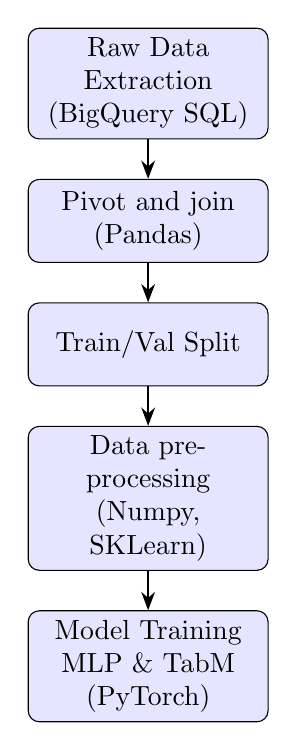
\begin{tikzpicture}[
      block/.style = {rectangle, draw, fill=blue!10,
                      text width=8em, align=center,
                      rounded corners, minimum height=3em},
      arrow/.style = {-{Stealth}, thick},
      node distance=.5cm
    ]
    % Nodes
    \node[block] (extract) {Raw Data Extraction\\(BigQuery SQL)};
    \node[block, below=of extract] (merge) {Pivot and join\\(Pandas)};
    \node[block, below=of merge] (split) {Train/Val Split};
    \node[block, below=of split] (clean) {Data preprocessing\\(Numpy, SKLearn)};
    \node[block, below=of clean] (train) {Model Training\\MLP \& TabM (PyTorch)};

    % Arrows
    \draw[arrow] (extract) -- (merge);
    \draw[arrow] (merge)   -- (split);
    \draw[arrow] (split)   -- (clean);
    \draw[arrow] (clean)   -- (train);
  \end{tikzpicture}
  \caption{End‐to‐end biological‐age pipeline: from raw MIMIC-IV extraction to model evaluation.}
  \label{fig:pipeline}
\end{figure}


\section{Results}
\label{sec:results}

Our experiments demonstrate that the proposed TabM architecture significantly improves prediction accuracy over a simple multilayer perceptron (MLP) baseline.  All errors are reported as unscaled root–mean–square error (RMSE) in years, obtained by back‐transforming the model outputs using the target population mean (62.67 years) and standard deviation (16.18 years).

\subsection{Predictive Performance}
\begin{table}[ht]
  \centering
  \begin{tabular}{lcc}
    \toprule
    Model                                   & RMSE (years) & Improvement vs.\ MLP \\
    \midrule
    MLP (continuous only)                   & 11.28        & ---                  \\
    TabM (continuous only)                  & 11.04        & 2.1\%               \\
    TabM (continuous + categorical)         &  9.24        & 18.1\%              \\
    \bottomrule
  \end{tabular}
  \caption{Comparison of unscaled RMSE for age prediction models.}
  \label{tab:rmse_comparison}
\end{table}

\subsection{Variance Explained}

By comparing unscaled MSE to the total variance of chronological age ($\sigma^2 = 16.1793^2 \approx 261.8$):
\[
  R^2 \;=\; 1 - \frac{(9.23)^2}{261.8} \;\approx\; 0.67,
\]
indicating that our best model explains approximately 67\% of the variation in patient age.

\subsection{Summary of Results}

These results demonstrate that parameter‐efficient ensembling (TabM) yields modest gains over a basic MLP when using only continuous laboratory and chart features, and that incorporating key categorical demographics further boosts accuracy by nearly two years of RMSE. This level of precision ($\approx9.2$ years) represents a substantial advance toward practical biological‐age estimation from routine clinical data.

\begin{figure}[ht]
\centering
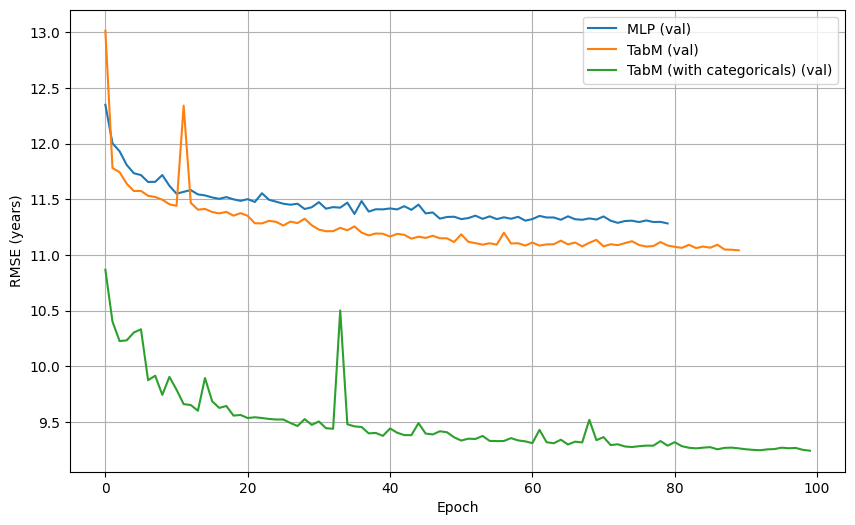
\includegraphics[width=\linewidth]{hrp.png}
\caption{Model loss over training epochs on the validation set.}
\label{fig:workflow}
\end{figure}


\section{Conclusion}

In this work, we developed a lightweight biological‐age predictor using routinely collected laboratory and demographic data from MIMIC-IV. By comparing a simple multilayer perceptron (MLP) baseline to our parameter‐efficient TabM model and its extension incorporating categorical covariates, we demonstrated progressive improvements in validation RMSE—from 11.28 years (MLP) to 11.04 years (TabM) and finally to 9.24 years (TabM + categoricals). These results illustrate that efficient ensembling of MLPs can yield highly accurate age estimates without resorting to expensive or high‐dimensional omics data.

Future work can explore several avenues for enhancing and extending this approach:
\begin{itemize}
  \item \textbf{Interpretability and feature importance:} Apply model‐agnostic methods (e.g., SHAP) to identify the most informative biomarkers and improve clinical trust.
  \item \textbf{Uncertainty quantification:} Leverage the ensemble nature of TabM to derive prediction intervals and support decision‐making in individual patients.
  \item \textbf{Temporal modeling:} Extend the pipeline to predict \emph{biological age acceleration} and its longitudinal trajectories using recurrent or attention‐based architectures.
  \item \textbf{External validation:} Test the model on other hospital systems or population cohorts to assess generalizability and robustness.
\end{itemize}

Overall, our findings highlight the promise of efficient deep‐learning ensembles for scalable, cost‐effective biological‐age estimation and lay the groundwork for richer, clinically actionable models in the future.

%%
%% The next two lines define the bibliography style to be used, and
%% the bibliography file.
\bibliographystyle{ACM-Reference-Format}
\bibliography{references}

\end{document}
\endinput
%%
%% End of file `sample-manuscript.tex'.
